%%%%%%%%%%%%%%%%%%%%%%%%%%%%%%%%%%%%%%%%%
% Journal Article
% LaTeX Template
% Version 1.1 (25/11/12)
%
% This template has been downloaded from:
% http://www.LaTeXTemplates.com
%
% Original author:
% Frits Wenneker (http://www.howtotex.com)
%
% License:
% CC BY-NC-SA 3.0 (http://creativecommons.org/licenses/by-nc-sa/3.0/)
%
%%%%%%%%%%%%%%%%%%%%%%%%%%%%%%%%%%%%%%%%%

%----------------------------------------------------------------------------------------
%   PACKAGES AND OTHER DOCUMENT CONFIGURATIONS
%----------------------------------------------------------------------------------------

%\documentclass[twoside]{article}
\documentclass[10pt]{article}

\usepackage[english]{babel}
\usepackage{graphicx}

\usepackage{lipsum} % Package to generate dummy text throughout this template

\usepackage[sc]{mathpazo} % Use the Palatino font
\usepackage[T1]{fontenc} % Use 8-bit encoding that has 256 glyphs
\linespread{1.05} % Line spacing - Palatino needs more space between lines
\usepackage{microtype} % Slightly tweak font spacing for aesthetics

\usepackage{url}

\addtolength{\oddsidemargin}{-.875in}
\addtolength{\evensidemargin}{-.875in}
\addtolength{\textwidth}{1.75in}
\addtolength{\topmargin}{-.875in}
\addtolength{\textheight}{1.75in}

\usepackage[hmarginratio=1:1,top=26mm,columnsep=20pt]{geometry} % Document margins
\usepackage{multicol} % Used for the two-column layout of the document
\usepackage{hyperref} % For hyperlinks in the PDF

\usepackage[hang, small,labelfont=bf,up,textfont=it,up]{caption} % Custom captions under/above floats in tables or figures
\usepackage{booktabs} % Horizontal rules in tables
\usepackage{float} % Required for tables and figures in the multi-column environment - they need to be placed in specific locations with the [H] (e.g. \begin{table}[H])

\usepackage{lettrine} % The lettrine is the first enlarged letter at the beginning of the text
\usepackage{paralist} % Used for the compactitem environment which makes bullet points with less space between them

\usepackage{abstract} % Allows abstract customization
\renewcommand{\abstractnamefont}{\normalfont\bfseries} % Set the "Abstract" text to bold
\renewcommand{\abstracttextfont}{\normalfont\small\itshape} % Set the abstract itself to small italic text

\usepackage{titlesec} % Allows customization of titles
%\renewcommand\thesection{\Roman{section}}
\titleformat{\section}[block]{\large\scshape\centering}{\thesection.}{1em}{} % Change the look of the section titles

%\usepackage{fancyhdr} % Headers and footers
%\pagestyle{fancy} % All pages have headers and footers
%\fancyhead{} % Blank out the default header
%\fancyfoot{} % Blank out the default footer
%\fancyhead[C]{Running title $\bullet$ November 2012 $\bullet$ Vol. XXI, No. 1} % Custom header text
%\fancyfoot[RO,LE]{\thepage} % Custom footer text

%----------------------------------------------------------------------------------------
%   TITLE SECTION
%----------------------------------------------------------------------------------------

\title{\vspace{-15mm}\fontsize{24pt}{10pt}\selectfont\textbf{LUMP: Locking and Unlocking Mobile Platform}} % Article title

\author{
    \large
    \textsc{Mason Silber \quad Vivek Bhagwat}\\[2mm] % Your name
    \normalsize Columbia University \\ % Your institution
    \normalsize \{mds2161,vsb2110\}@columbia.edu % Your email address
    \vspace{-5mm}
}
\date{}

%----------------------------------------------------------------------------------------

\begin{document}

\maketitle % Insert title

%\thispagestyle{fancy} % All pages have headers and footers

%----------------------------------------------------------------------------------------
%   ARTICLE CONTENTS
%----------------------------------------------------------------------------------------

\begin{multicols}{2} % Two-column layout throughout the main article text

%----------------------------------------------------------------------------------------
%   ABSTRACT
%----------------------------------------------------------------------------------------

\begin{abstract}

While a great deal of research has gone into software-based security on mobile devices, the technologies of hardware and software have not been combined to work together. Furthermore, even with the explosion of mobile computing in the last decade, there have been few mainstream implementations of systems that leverage mobile devices to control physical locks. With an iOS application, an Arduino Uno, a servo motor, and a Raspberry Pi, we leverage technologies such as SSL and Firmata to allow for secure connections from a mobile app to engage mechanical latches which act as locks.

\end{abstract}

\section{Introduction}
Locks may be one of the most pervasive technologies in the world. Traditional, physical locks are used for houses, cars, windows, fences, and luggage --- every object in the world humans deem worth protecting. However, it was not always just objects themselves that were worth protecting --- it was information as well.\\

There are a few examples of this type of information security --- the first is physically protecting information by putting it in a safe with a dial \cite{safestructure}, such that turning the dial the correct amount in the correct direction a few times in sequence allows access to the contents of a box. This design allows for physical valuables to be stored in such a way that makes it only accessible to those who have knowledge of the correct sequence of physical manipulations of a lock. \\

The second type, which is more relevant in our increasingly electronic world, is the obfuscation of information through means such as ciphers, which encodes information in such a way that can only be decoded if the reader knows the algorithm, or cipher, which allows them to change the form into a human-readable format. This method is much older than the computing technology ubiquitous today, however. Classical ciphers, for example, simply substitute letters with other letters (e.g. $G$ could be always replaced with $L$). However, the problems with this sort of cipher is that it is easy to figure out an algorithm when it is simple and efficient to calculate, either by human or computer. This is the motivation behind symmetric and asymmetric encryption, which drives a great deal of authentication today. \\

Symmetric-key encryption algorithms are ones in which the same key is used for both encryption and decryption \cite{cryptography}. This means that this key must be present for both the reader and writer, and agreed upon in advance. However, if the key is sufficiently complex, this allows for a simple and quick algorithm which still is inefficient and difficult to decipher for any third parties. Today, algorithms such as the Advanced Encryption Standard (AES) employ this form of encryption \cite{aes}. The main problem, however, is that both parties must know the key in advance. This makes AES perfectly acceptable for situations in which data are simply being encrypted for reading later, not transferred securely. \\

When transferring data over a medium which another party could potentially read, asymmetric-key encryption is preferred. Asymmetric-Key encryption is system in which users are able to share a ``public key'' insecurely with the intended recipient of some encrypted data \cite{ssl}. Additionally, a ``private key'' is generated for each of the two parties involved in the transfer such that the keys can be combined to make the data only readable to those who have the correct private and public key. This algorithm prevents anyone who has access to all data being transferred to be able to decrypt the data, because that user's private key will not be able to combine with the public key which has been distributed to allow access to the encrypted data. This type of encryption is pervasive across many types of systems, including HTTPS, which uses SSL with HTTP \cite{ssl}.  It is this implementation of asymmetric-key encryption that is relevant to this paper. \\

In the physical world, however, we cannot simply use numbers to protect our valuables. This is the reasons safes still exist and are so widely used, and is one of the motivations of this project --- to combine the convenience of software security and the protection of lockboxes. Traditionally, identity can be verified in some subset of ``what you know,'' ``what you have,'' and ``what you are.''  \cite{codinghorror} Software security implementations as described above generally rely on the ``what you know'' aspect (e.g. passwords, public and private keys, etc.) of identity verification while traditional locks rely on ``what you have'' (i.e. physical keys for a physical lock). As a result, companies  such as Google, Dropbox \cite{dropboxtwostep}, and Twitter \cite{twittertwostep} have recently begun implementing two-step verification for logging into their services. These verification processes usually rely on knowledge of a password as well as ownership of a smartphone, which provides a temporal code which can be entered into the service as a second step in the authentication process. \\

The ability to rely on both these forms of identity verification allows for a more robust security system, and the ubiquity of technologies such as smartphones makes these implementations have far-reaching effects.\\

\section{Overview of iOS and Arduino and Raspberry Pi}

\subsection{iOS}

iOS is a closed-source, mobile operating system developed by Apple, Inc., and is one of the most popular mobile operating systems in the world. iOS runs on iPhone, iPod, iPad, and AppleTV; as of June 2012, over 400 million devices worldwide were running iOS. \cite{applenums}\\

iOS architecture has an architecture made up of four layers \cite{iosoverview}. The top layer is Cocoa Touch, which provides developers with standardized user interface objects such as buttons, sliders, table views, and other commonly used components \cite{cocoatouch}. Cocoa Touch also provides abstractions from lower-level functionality in a number of frameworks. Native frameworks exist for audio processing, animation and graphics development, networking, and persistent storage, among others. As its name suggests, Cocoa Touch also provides access to all touch events that occur on the device.\\

\begin{figure}[H]
\centering
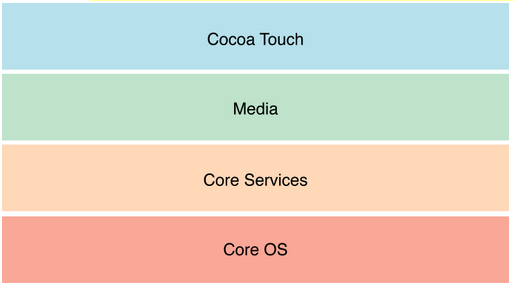
\includegraphics[width=0.5\textwidth]{ios_arch.png}
\caption{iOS Architecture \cite{iosoverview}}
\end{figure}
 
The next layer is the Media layer \cite{iosmedia}. The media layer provides lower level access to audio, video, graphics, and animation functionality and processing. Frameworks such as Core Text, Core Image, Core MIDI, and GLKit exist in this layer. \\

Below the Media layer is the Core Services layer \cite{ioscoreservices}. Core Services provides access to iCloud technologies, a system by which user information and data can be automatically synced in the cloud using key-value storage. The Core Services layer also facilitates Automatic Reference Counting, relieving developers of most of the responsibility of memory management. Core Services provides developers with the ability to pass blocks of code as function parameters. This functionality allowed for the implementation of a C library called Grand Central Dispatch (GCD), which makes multithreaded app development much simpler. Frameworks like the Accounts Framework (access to Twitter and Facebook), the Ad Support Framework, and the Foundation Framework. \\

The last layer of the iOS architecture is the Core OS layer \cite{ioscoreos}. Core OS provides access to external hardware attachments and internal hardware components, such as the bluetooth receiver and the accelerometer. The Core OS layer also provides developers with security libraries and basic access to system calls. \\

\begin{figure}[H]
\centering
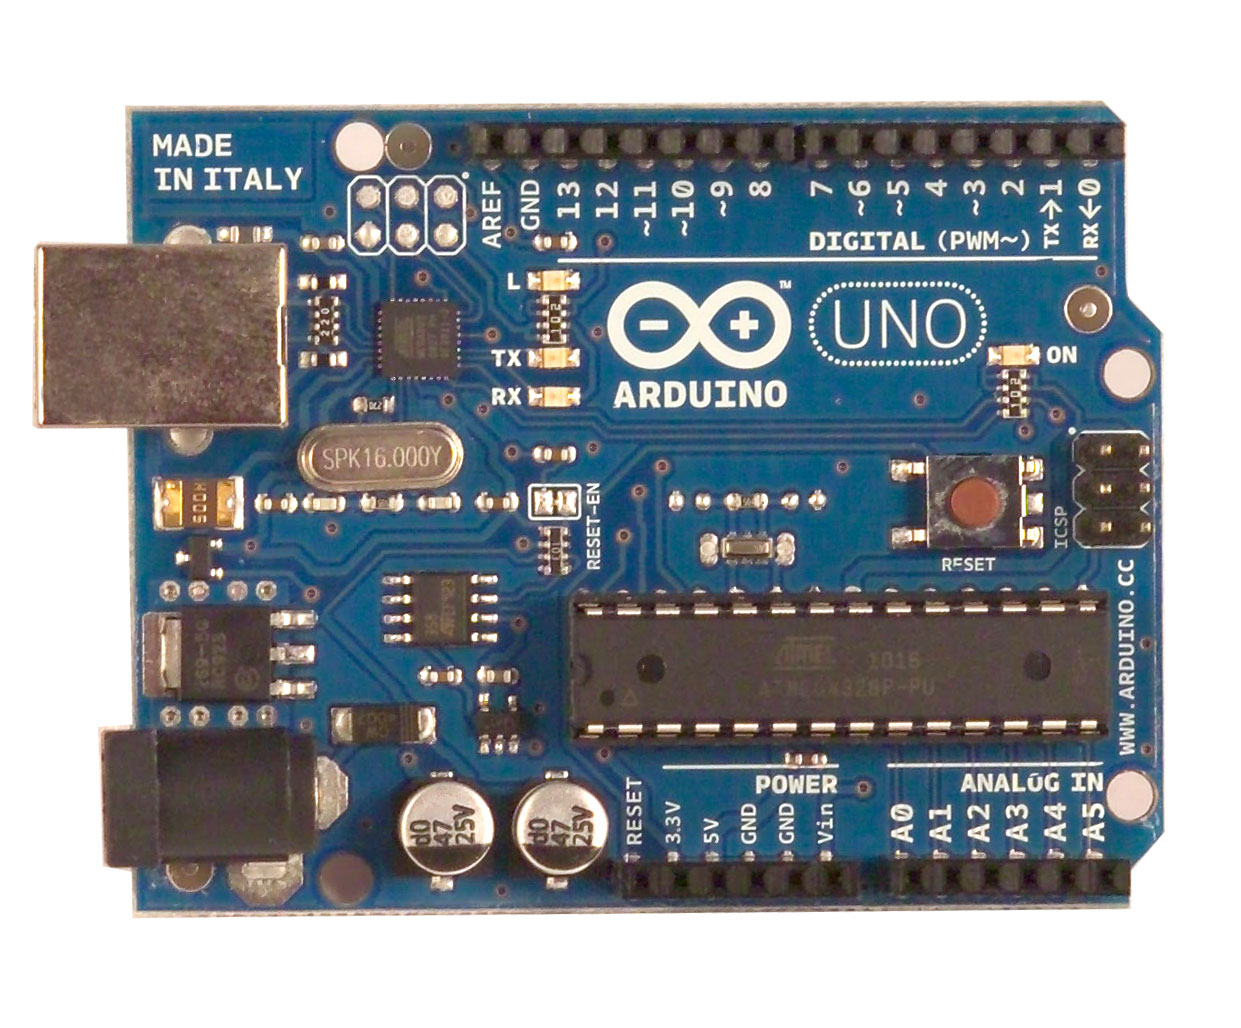
\includegraphics[width=0.5\textwidth]{arduino.jpg}
\caption{Arduino Uno}
\end{figure}

\subsection{Arduino Uno}
Arduino is an open-source microcontroller designed with the intention of making hardware development more accessible \cite{arduinoschematic}. Because we used an Arduino Uno in our experimental setup, we will limit our discussion to that particular model. \\

The Arduino Uno \cite{arduinouno} is a board designed around the ATmega328 microcontroller. It has 32 kb of flash memory, 2 kb of SRAM, and 1 kb of EEPROM. There are 14 digital I/O pins and 6 analog in pins, which can be controlled or read by the microcontroller. Six of the digital I/O pins are also able to emit Pulse Width Modulated (PWM) signals, which are used to control motors and other components. The Arduino is powered with a 5V power supply, either from a USB port or an AC to DC converter. \\

However, what truly differentiates Arduino from other microcontrollers is the presence of a bootloader. Whereas normal microcontrollers often need an external programmer to load a program onto the chip before it is placed on the circuit board, Arduino's bootloader allows C programs to be uploaded directly from the developer's machine to the microcontroller's flash memory. This allows the code to be executed immediately, and streamlines development. \\

Aside from loading programs directly into the microcontroller's flash memory, serial directives can be sent over USB to the Arduino using a protocol called Firmata. We use this approach in our experimental design with our secure server, which handles user requests. \\

\subsection{Raspberry Pi}
The Raspberry Pi \cite{raspberrypi} is an open source, low cost, single board computer developed by the Raspberry Pi Foundation. Two models currently exist, Model A and Model B. We used a Model B Raspberry Pi in our experimental setup, so we will not discuss Model A. \\

\begin{figure}[H]
\centering
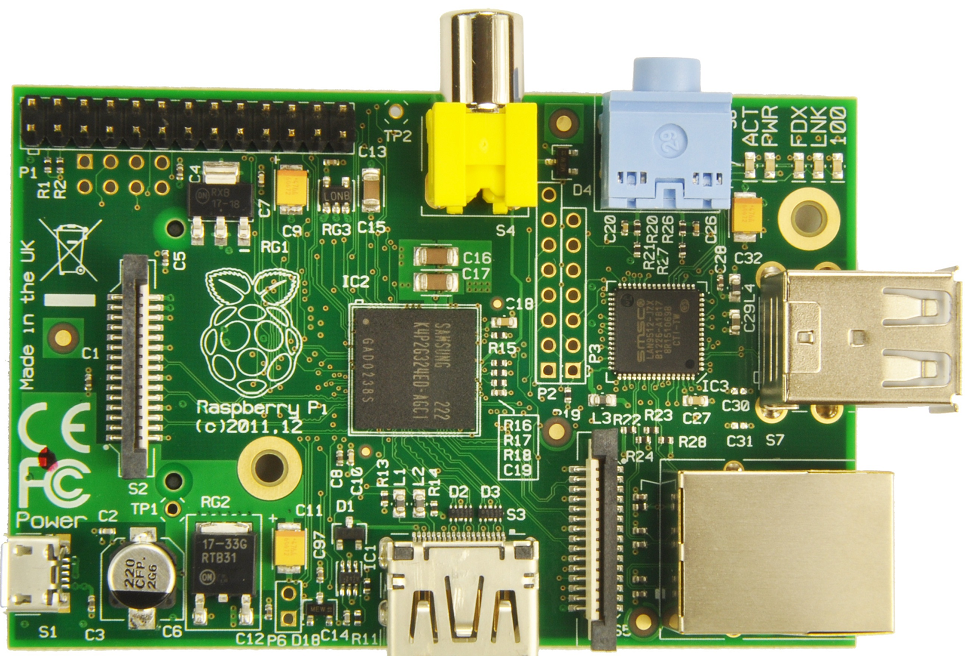
\includegraphics[width=0.5\textwidth]{raspberrypi.png}
\caption{Raspberry Pi Model B}
\end{figure}

At a price of just \$35, the Model B Raspberry Pi is one of the cheapest computers on the market. It ships with an 800MHz ARM processor, 512 MB of RAM, audio and video out, an Ethernet jack, two USB ports, an HDMI port, 26 GPIO pins, and an SD card slot. It runs many distributions of Linux, including Arch Linux ARM, Debian, Fedora, and others. For this project we chose to use Raspbian OS, a distribution of Debian designed specifically for the Raspberry Pi. \\

\subsection{Firmata}
Firmata \cite{firmatawiki} is an open-source protocol used to communicate between a computer and a microcontroller. The computer sends serial data via USB (or some other connector) to the microcontroller, and receives serial data in response. Firmata allows microcontrollers to be significantly augmented by much more powerful computers, and can be very useful in situations in which some heavy computation is being performed. \\

Libraries \cite{firmata} exist to communicate with Arduino through Firmata in many languages, including Perl, Python, Ruby, Java, and Javascript. All of these libraries are open source as well, and abstract away many of the low level difficulties associated with Firmata. \\

\subsection{BreakfastSerial}
BreakfastSerial \cite{breakfastserial} is an open-source Python library that facilitates serial communication between a computer and an Arduino through Firmata. BreakfastSerial includes abstractions for Arduino boards, LEDs, push button switches, RGB LEDs, Sensors, and Servo Motors. During our work on this project, we actually contributed to BreakfastSerial by implementing the abstraction for the Servo component, which we needed for our experimental setup. \\

Normally, Arduino programming must be done in C, a barrier which many people find tough to breach. Libraries like BreakfastSerial alleviate people of this responsibility by creating a way to develop for Arduino in higher level languages. In our experiment, we created a Python HTTPS server to handle locking and unlocking requests, so BreakfastSerial is an ideal library for our purposes. \\

\begin{figure}[H]
\centering
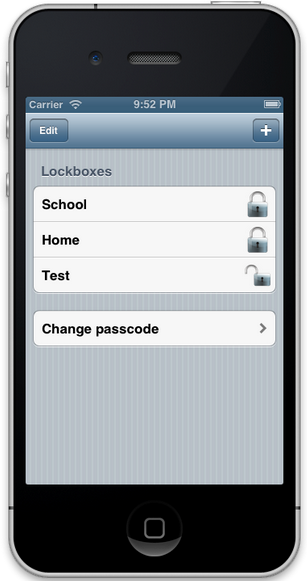
\includegraphics[height=3in]{ios.png}
\caption{Lockbox Home Screen}
\end{figure}

\section{Experimental Setup}

\subsection{Client Side}

Our client application is an iOS app, titled Lockbox. Lockbox is a very simple app that lists a user's locks and whether each lock is currently locked or unlocked. The app also facilitates in-app additions of new locks, using a single, simple form. \\

Lockbox launches by prompting the user to enter a four digit PIN, in order to access their locks. If this is the first time the app is being launched, the user will be required to input a four digit PIN, which is stored securely in the iPhone's keychain. \\

Upon a successful entry of the PIN, the app launches into the home screen, which is simply a list of locks that the user has added to the app and each lock's status. Users can at any point edit or remove a lock simply by hitting the ``Edit'' button in the top left hand corner. Users can also add a new lock by hitting the ``+'' button in the top right corner. To lock or unlock a lock, a user simply taps that lock's entry and a request is immediately sent to the server through HTTPS. \\

Hitting the ``+'' button brings the user to a form with only two fields: lock name and lock IP address. Once these things are entered and ``Save'' is tapped, this lock is placed in secure persistent storage through a SQLite wrapper provided by Apple called Core Data. Along with the name and IP address, Core Data stores a randomly generated string that serves as an identifier for that particular lock. The server listening for requests being made to that lock will not serve any request that does not contain that identifier as one of its parameters. \\

One thing to note is that all networking requests are performed using the external library AFNetworking \cite{afnetworking}. AFNetworking provides a powerful wrapper around the native iOS networking classes, and makes things like basic authentication and HTTPS requests much simpler than they would be with the libraries built into iOS. AFNetworking requests allow blocks of code to be passed into network request function calls, to be executed on a successful or a failed request. This proved to be particularly useful for is, because knowing the current status of the lock at any point in time is the crux of our experiment. \\

\subsection{Server Side}
\begin{figure}[H]
\centering
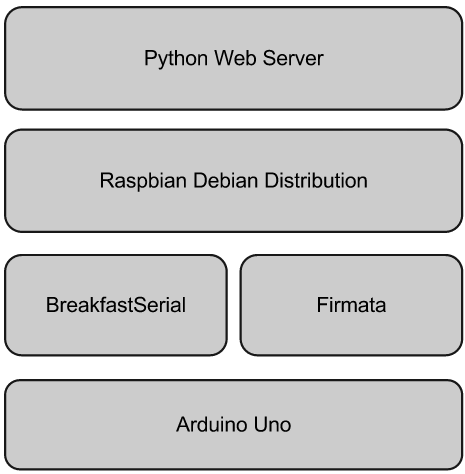
\includegraphics[width=0.5\textwidth]{stack.png}
\caption{Server Side architecture}
\end{figure}

The server side architecture is made up of a couple of different layers. The top layer is a Python server that only accepts HTTPS requests, in order to ensure security. The server simply listens for locking, unlocking, and creation requests. Upon receiving a request, it checks the parameters of the request to ensure that the proper identifier for that particular lock has been passed. The server also sends serial information to the hardware when processing the requests, which will be discussed in more detail below. \\

The server uses two python libraries in conjunction, \texttt{ssl} \cite{pyssl} and \texttt{BaseHTTPServer} \cite{BaseHTTPServer}, which enable a basic http server to run with an ssl socket enabled. With this, we are able to keep this server running and accepting connections, but only responding to secure requests such that the metadata sent with each request cannot be seen by third parties. \\

The server itself runs on a Raspberry Pi Model B using Python 2.7.3. The Raspberry Pi runs Raspbian \cite{raspbian}, a particular Debian distribution designed with the hardware constraints of the Raspberry Pi in mind, and comes pre-installed with Python on it. This feature combined with the simplicity of Python as a programming language made the Raspberry Pi a particularly good computer on which we could run our server. The integration of the Raspberry Pi in the hardware design of the experiment will be discussed the next section. \\

The server utilizes a python library called BreakfastSerial, discussed above. When a request is received, the server processes it, and if the request had the proper identifier in its parameters, it will send serial information to the two status indicator LEDs and to the servo motor, which controls the turning mechanism of the lock and is at the heart of the electromechanical piece of the experiment. \\

Lastly, the Arduino Uno is connected via USB to the Raspberry Pi, and has been preloaded with a program that comes with the Arduino IDE called StandardFirmata, built on the Arduino Firmata library \cite{arduinofirmata}. StandardFirmata makes the Arduino listen for serial commands from the server via USB, such as toggling LEDs or turning the servo. The only downside to this is that it requires a wired connection; however, because of the small size of both the Raspberry Pi and the Arduino, this issue is inconsequential. \\

\subsection{Hardware}

The hardware apparatus for this experiment was not particularly complex because of the simplicity both the Raspberry Pi and the Arduino afforded. The Raspberry Pi is powered by a 5V power supply in the form of either an AC/DC micro USB power supply plugged into the wall or a set of batteries and a voltage regulator. The Raspberry Pi also needs some form of network connection; this can be achieved most easily with an Ethernet Cable, as the Raspberry Pi has a CAT5 port, but a USB Wifi dongle could work as well. Because the lock was supposed to be completely wireless, we decided to use the solution involving the batteries, voltage regulator, and Wifi dongle, as opposed to a power supply and an Ethernet cable. The last component connected to the Raspberry Pi is a USB A-to-B serial cable, which connects the Arduino to the Raspberry Pi and carries instructions from the server to the lock. \\

\begin{figure*}[t!]
\centering
%\includegraphics[width=0.5\textwidth]{circuit.png}
\includegraphics[height=3.5in]{circuit.png}
\caption{Circuit}
\end{figure*}

The Arduino has a number of components which it controls. Pins 4 and 5 connect to a tri-color LED, which indicates whether a network connection is available or not. If not, the server cannot receive requests. Pin 4 triggers the red LED within the tri-color LED, signaling no network connection, and pin 5 triggers the blue LED within the tri-color LED, signaling successful connection to the network. Pins 6 and 7 also control a status indicating tri-color LED, which indicates whether the lock is locked or unlocked. Pin 6 triggers the red LED, and is turned on when the lock is locked, and pin 7 triggers the green LED, which is activated when the lock is unlocked. Both tri-color LEDs are connected to ground via two 100 $\Omega$ resistors. \\

The servo motor connects to the Arduino through three different wires. One wire goes directly to the 5V power supply, one goes directly to ground, and one goes to pin 10. Pin 10 controls the pulse width modulation, and therefore the position of the servo. The servo's position is completely determined by the width of the pulse going through the pin at any given time, which is in turn controlled by what value the server writes to it. \\


\section{Results}
We implemented a fully-featured iPhone app as well as the secure HTTPS Python server interfaced with BreakfastSerial. The iPhone app's communication with the Python server was virtually instantaneous (though this could be attributed to particular network speeds), and locks were encrypted and secured both locally on the iPhone and remotely on the corresponding server. Though it functioned correctly on an Ubuntu virtual machine, there were some issues \cite{breakfastserialissue} with the serial connection or the drivers when communicating with the Arduino from the Raspberry Pi via BreakfastSerial, as documented on Github. 

\section{Related Work}
Wireless networked security has become a popular entrepreneurial venture in the last few years. Many companies have announced locks you can control with a remote, from your phone, or simply by walking up to the door. \\

One of the most notable companies to market a similar product is Lockitron \cite{lockitron}. Lockitron provides a wireless electronic lock for normal doors. Controlled via a smartphone app or a text message, Lockitron locks allow users to lock and unlock their doors from anywhere, get notifications whenever their door is locked or unlocked, distribute expiring keys (bed and breakfasts may use this, for example). \\

However, Lockitron's solution costs \$179 to pre order, and only works for doors. Our solution addresses a more general problem. Our implementation could be used on doors as well, but also on safes, lock boxes, cars, and anything else with a locking and unlocking mechanism. The simplicity of the servo implementation allows for easy, adaptable extensions for locks on nearly anything.\\

\section{Conclusions}
Though a universal solution has not been implemented to solve this problem, it's clear that a platform like LUMP would be of great use in many situations to a diverse set of users. This solution is easily extendable to the Android and Windows Phone platforms as well, creating an even larger market for such a product. 

\section{Future Work}
Though LUMP has most of its components working together, improvements could be made in three specific areas. The first is the mobility and adaptability of the device, the second is more physical, such that our lock ensures better physical security, and the third is better software security in terms of actual data storage.\\

With regard to mobility and adaptability, the connection between the server and the Arduino was not fully functional when the server was running on Raspberry Pi \cite{breakfastserialissue}. The connection was inconsistent and often failed for reasons we failed to completely debug. As a result, the solution relied on a more traditional laptop running a server --- an overhead that is unnecessary in both physical and fiscal cost. With the raspberry pi working, the solution would be more mobile.\\

The problem with using the latch in the way we did with one small servo is that the latch is not necessarily physically very strong. This is an obvious problem with our prototype, but not a problem with our overall solution. The adaptable nature of LUMP allows for stronger servos and latches to be attached to the arduino, with power being the only limitation.\\

The third, software-based solution would be to put more research into secure storage on the server-side. Currently, no encryption is performed on the keys and lockbox ids, only on the calls which initially pass them to the server from the iOS app. Less focus was put into this because we were more concerned with the potential physical security issues than any software based issues which would rely on file access. Ideally, the data would be stored not on the server at all but for the purposes of this prototype we were more concerned with the mechanics of a secure request to result directly affecting a physical lock. These issues are all likely solvable, and would be necessary before any commercial implementation was pursued.\\


\section{Acknowledgments}
We would like to thank Professor Jason Nieh for the advice and guidance he has provided for us throughout the semester with regards to our project. We would also like to thank Swift \cite{swift} for accepting our pull request on BreakfastSerial and for helping us implement the Servo component for the BreakfastSerial module. Lastly, we would like to thank the Columbia University Electrical Engineering department for lending us electronics components when we needed them, and eBay for providing a platform through which to buy cheap, mass produced electronics. 



%------------------------------------------------


%----------------------------------------------------------------------------------------
%   REFERENCE LIST
%----------------------------------------------------------------------------------------

\begin{thebibliography}{99} % Bibliography - this is intentionally simple in this template
  
  \bibitem{afnetworking}
  "AFNetworking." Github. \url{https://github.com/AFNetworking/AFNetworking} (accessed May 13, 2004).

\bibitem{aes}
"Announcing the Advanced Encryption Standard." Federal Information Processing Standards. \url{http://www.google.com/url?q=http\%3A\%2F\%2Fcsrc.nist.gov\%2Fpublications\%2Ffips\%2Ffips197\%2Ffips-197.pdf&sa=D&sntz=1&usg=AFQjCNHW4yah4ynS8KuVEfHO77pwcvrxLQ} (accessed May 4, 2013).

\bibitem{arduinouno}
"Arduino - ArduinoBoardUno ." Arduino. \url{http://arduino.cc/en/Main/ArduinoBoardUno} (accessed May 4, 2013).

\bibitem{arduinoschematic}
"Arduino Uno Rev3 Schematic." Arduino. \url{arduino.cc/en/uploads/Main/Arduino_Uno_Rev3-schematic.pdf} (accessed May 13, 2004).

\bibitem{breakfastserial}
"BreakfastSerial." Github. \url{https://github.com/theycallmeswift/BreakfastSerial} (accessed May 13, 2004).

\bibitem{breakfastserialissue}
"BreakfastSerial Issues." Github. \url{https://github.com/theycallmeswift/BreakfastSerial/issues/3} (accessed May 13, 2004).

\bibitem{cocoatouch}
"Cocoa Touch." Apple Developer. \url{https://developer.apple.com/technologies/ios/cocoa-touch.html} (accessed May 13, 2004).

\bibitem{dropboxtwostep}
D'Orazio, Dante. "Dropbox two-step verification security option to lock down your files available now (update) | The Verge." The Verge. \url{http://www.theverge.com/2012/8/26/3269423/dropbox-two-step-verification-security-beta} (accessed May 4, 2013).

\bibitem{cryptography}
Delfs, Hans, and Helmut Knebl. "Introduction to Cryptography: Principles and Applications - Hans Delfs, Helmut Knebl - Google Books." Google Books. \url{http://books.google.com/books?id=Nnvhz_VqAS4C&pg=PA11#v=onepage&q&f=false} (accessed May 4, 2013).


\bibitem{firmata}
"Firmata Arduino Libraries." Github. \url{https://github.com/firmata/arduino} (accessed May 13, 2004).

\bibitem{raspbian}
"FrontPage - Raspbian." Raspbian. \url{http://www.raspbian.org/} (accessed May 4, 2013).

\bibitem{twittertwostep}
Honan, Mat. "Twitter Now Has a Two-Step Solution | Threat Level | Wired.com." wired.com . \url{http://www.wired.com/threatlevel/2013/04/twitter-authentication/} (accessed May 4, 2013).

\bibitem{nieh}
"Jason Nieh." Department of Computer Science, Columbia University | Home. \url{http://www.cs.columbia.edu/~nieh/} (accessed May 4, 2013).

\bibitem{lockitron}
"Lockitron." Lockitron. \url{https://lockitron.com/} (accessed May 13, 2004).

\bibitem{firmatawiki}
"Main Page - Firmata." Firmata. \url{http://firmata.org/wiki/Main_Page} (accessed May 4, 2013).

\bibitem{safestructure}
"Patent US1838581 - SAFE STRUCTURE - Google Patents." Google. \url{http://www.google.com/patents/US1838581} (accessed May 4, 2013).

\bibitem{ssl}
"SSL/TLS Strong Encryption: An Introduction - Apache HTTP Server." The Apache HTTP Server Project. \url{http://httpd.apache.org/docs/2.2/ssl/ssl_intro.html#cryptographictech} (accessed May 4, 2013).

\bibitem{applenums}
Sloan, Paul. "Apple by the numbers: 84M iPads, 400M iOS devices, 350M iPods sold | Apple - CNET News." Technology News - CNET News. \url{http://cnet.co/OHaJs5} (accessed May 4, 2013).

\bibitem{swift}
"SwiftAlphaOne's Twitter Account." Twitter. \url{https://twitter.com/swiftalphaone} (accessed May 13, 2004).

\bibitem{arduinofirmata}
analogPin;, te. "Arduino - Firmata ." Arduino. \url{http://arduino.cc/en/Reference/Firmata} (accessed May 4, 2013).

\bibitem{raspberrypi}
"FAQs  | Raspberry Pi." Raspberry Pi | An ARM GNU/Linux box for \$25. Take a byte!. \url{http://www.raspberrypi.org/faqs} (accessed May 4, 2013).

\bibitem{iosoverview}
"iOS Technology Overview." Apple Developer. \url{developer.apple.com/library/ios/#documentation/Miscellaneous/Conceptual/iPhoneOSTechOverview/Introduction/Introduction.html} (accessed May 13, 2004).

\bibitem{ioscoreservices}
"iOS Technology Overview: Core Services Layer." Apple Developer. \url{developer.apple.com/library/ios/#documentation/miscellaneous/conceptual/iphoneostechoverview/CoreServicesLayer/CoreServicesLayer.html} (accessed May 13, 2004).

\bibitem{ioscoreos}
"iOS Technology Overview: CoreOS Layer." Apple Developer. \url{developer.apple.com/library/ios/#documentation/miscellaneous/conceptual/iphoneostechoverview/coreoslayer/coreoslayer.html} (accessed May 13, 2004).

\bibitem{iosmedia}
"iOS Technology Overview: Media Layer." Apple Developer. \url{developer.apple.com/library/ios/#documentation/miscellaneous/conceptual/iphoneostechoverview/MediaLayer/MediaLayer.html} (accessed May 13, 2004).

\bibitem{codinghorror}
Atwood, Jeff. "Coding Horror: What You Have, What You Know, What You Are." Coding Horror. \url{http://www.codinghorror.com/blog/2007/02/what-you-have-what-you-know-what-you-are.html} (accessed May 4, 2013).

\bibitem{BaseHTTPServer}
"20.18. BaseHTTPServer --- Basic HTTP server --- Python v2.7.4 documentation." Overview --- Python v2.7.4 documentation. http://docs.python.org/2/library/basehttpserver.html (accessed May 5, 2013).

\bibitem{pyssl}
tes. "17.3. ssl --- TLS/SSL wrapper for socket objects --- Python v2.7.4 documentation." Overview --- Python v2.7.4 documentation. http://docs.python.org/2/library/ssl.html (accessed May 5, 2013).



\end{thebibliography}

%----------------------------------------------------------------------------------------

\end{multicols}

\end{document}

